% configurações




\documentclass[
	% -- opções da classe memoir --
	12pt,				% tamanho da fonte
	openright,			% capítulos começam em pág ímpar (insere página vazia caso preciso)
	oneside,			% para impressão em recto e verso. Oposto a oneside
	a4paper,			% tamanho do papel. 
	% -- opções da classe abntex2 --
	%chapter=TITLE,		% títulos de capítulos convertidos em letras maiúsculas
	%section=TITLE,		% títulos de seções convertidos em letras maiúsculas
	%subsection=TITLE,	% títulos de subseções convertidos em letras maiúsculas
	%subsubsection=TITLE,% títulos de subsubseções convertidos em letras maiúsculas
	% -- opções do pacote babel --
	english,			% idioma adicional para hifenização
	french,				% idioma adicional para hifenização
	spanish,			% idioma adicional para hifenização
	brazil				% o último idioma é o principal do documento
	]{abntex2}




% Pacotes básicos 
\usepackage{lmodern}			% Usa a fonte Latin Modern			
\usepackage[T1]{fontenc}		% Selecao de codigos de fonte.
\usepackage[utf8]{inputenc}		% Codificacao do documento (conversão automática dos acentos)
\usepackage{indentfirst}		% Indenta o primeiro parágrafo de cada seção.
\usepackage{color}				% Controle das cores
\usepackage{graphicx}			% Inclusão de gráficos
\usepackage{microtype} 			% para melhorias de justificação
\usepackage{amsmath}			% lib para equacoes
\usepackage{svg}
%\usepackage{float}
\usepackage[T1]{fontenc}
\usepackage{listings}
\usepackage{tikz}
\usepackage{caption}
\usepackage{url}

\usepackage{titlesec}
\newcommand{\sectionbreak}{\clearpage}
\usepackage{hyperref}

\usetikzlibrary{shapes.geometric, arrows}

\tikzstyle{startstop} = [rectangle, rounded corners, 
minimum width=3cm, 
minimum height=1cm,
text centered, 
draw=black, 
fill=red!30]

\tikzstyle{io} = [trapezium, 
trapezium stretches=true, % A later addition
trapezium left angle=70, 
trapezium right angle=110, 
minimum width=3cm, 
minimum height=1cm, text centered, 
draw=black, fill=blue!30]


\tikzstyle{process} = [rectangle, 
minimum width=3cm, 
minimum height=1cm, 
text centered, 
text width=3cm, 
draw=black, 
fill=orange!30]

\tikzstyle{decision} = [diamond, 
minimum width=3cm, 
minimum height=1cm, 
text centered, 
draw=black, 
fill=green!30]
\tikzstyle{arrow} = [thick,->,>=stealth]



\definecolor{dkgreen}{rgb}{0,0.6,0}
\definecolor{gray}{rgb}{0.5,0.5,0.5}
\definecolor{mauve}{rgb}{0.58,0,0.82}

\lstset{frame=tb,
  language=Python,
  aboveskip=3mm,
  belowskip=3mm,
  showstringspaces=false,
  columns=flexible,
  basicstyle={\small\ttfamily},
  numbers=none,
  numberstyle=\tiny\color{gray},
  keywordstyle=\color{blue},
  commentstyle=\color{dkgreen},
  stringstyle=\color{mauve},
  breaklines=false,
  breakatwhitespace=false,
  upquote=true,
  tabsize=3
}

% Pacotes adicionais, usados apenas no âmbito do Modelo Canônico do abnteX2

\usepackage{lipsum}				% para geração de dummy text



% Pacotes de citações
\usepackage[num, backend=biblatex]{abntex2cite}	% Citações padrão ABNT
\usepackage[brazilian,hyperpageref]{backref}	 % Paginas com as citações na bibl

 
% CONFIGURAÇÕES DE PACOTES

% Configurações do pacote backref
% Usado sem a opção hyperpageref de backref
\renewcommand{\backrefpagesname}{Citado na(s) página(s):~}
% Texto padrão antes do número das páginas
\renewcommand{\backref}{}
% Define os textos da citação
\renewcommand*{\backrefalt}[4]{
	\ifcase #1 %
		Nenhuma citação no texto.%
	\or
		Citado na página #2.%
	\else
		Citado #1 vezes nas páginas #2.%
	\fi}%
% ---



% ---
% Informações de dados para CAPA e FOLHA DE ROSTO
% ---
\titulo{Robô omnidirecional de 3 rodas}
\autor{Daniel Ermelino Carvalho \\ Lucas Pereira Lima}
\local{Brasil}
\data{2024}
\orientador{Marcelo Bender Perotoni}
\instituicao{%
  Universidade Federal do ABC
  \par
  CECS
  \par
   Engenharia de Instrumentação, Automação e Robótica}
\tipotrabalho{Trabalho de graduação}
% O preambulo deve conter o tipo do trabalho, o objetivo, 
% o nome da instituição e a área de concentração 
\preambulo{Trabalho apresentado ao curso de engenharia de instrumentação,
automação e robótica da Universidade Federal do ABC como requisito parcial para
obtenção do título de bacharel em Engenharia de Instrumentação, Automação e 
Robótica.}



% Configurações de aparência do PDF final

% alterando o aspecto da cor azul
\definecolor{blue}{RGB}{5,5,180}

% informações do PDF
\makeatletter
\hypersetup{
     	%pagebackref=true,
		pdftitle={\@title}, 
		pdfauthor={\@author},
    	pdfsubject={\imprimirpreambulo},
	    pdfcreator={LaTeX with abnTeX2},
		pdfkeywords={abnt}{latex}{abntex}{abntex2}{trabalho acadêmico}, 
		colorlinks=true,       		% false: boxed links; true: colored links
    	linkcolor=blue,          	% color of internal links
    	citecolor=blue,        		% color of links to bibliography
    	filecolor=magenta,      		% color of file links
		urlcolor=blue,
		bookmarksdepth=4
}
\makeatother


% Posiciona figuras e tabelas no topo da página quando adicionadas sozinhas
% em um página em branco. Ver https://github.com/abntex/abntex2/issues/170
\makeatletter
\setlength{\@fptop}{5pt} % Set distance from top of page to first float
\makeatother



% Possibilita criação de Quadros e Lista de quadros.
% Ver https://github.com/abntex/abntex2/issues/176

\newcommand{\quadroname}{Quadro}
\newcommand{\listofquadrosname}{Lista de quadros}

\newfloat[chapter]{quadro}{loq}{\quadroname}
\newlistof{listofquadros}{loq}{\listofquadrosname}
\newlistentry{quadro}{loq}{0}

% configurações para atender às regras da ABNT
\setfloatadjustment{quadro}{\centering}
\counterwithout{quadro}{chapter}
\renewcommand{\cftquadroname}{\quadroname\space} 
\renewcommand*{\cftquadroaftersnum}{\hfill--\hfill}

\setfloatlocations{quadro}{hbtp} % Ver https://github.com/abntex/abntex2/issues/176


% Espaçamentos entre linhas e parágrafos 


% O tamanho do parágrafo é dado por:
\setlength{\parindent}{1.3cm}

% Controle do espaçamento entre um parágrafo e outro:
\setlength{\parskip}{0.2cm}  % tente também \onelineskip


% compila o indice
\makeindex



% Início do documento
\begin{document}

% Seleciona o idioma do documento (conforme pacotes do babel)
%\selectlanguage{english}
\selectlanguage{brazil}

% Retira espaço extra obsoleto entre as frases.
\frenchspacing 


% ELEMENTOS PRÉ-TEXTUAIS
	
% ---
% Capa
% ---
\imprimircapa
% ---

% ---
% Folha de rosto
% (o * indica que haverá a ficha bibliográfica)
% ---
\imprimirfolhaderosto
% ---



% ---
% inserir o sumario
% ---
\pdfbookmark[0]{\contentsname}{toc}
\tableofcontents*
\cleardoublepage
% ---


% ELEMENTOS TEXTUAIS
\textual

	% Introdução (exemplo de capítulo sem numeração, mas presente no Sumário)
	\chapter{Introdução}
	

Hello, here is some text without a meaning...



	% Capitulo com exemplos de comandos inseridos de arquivo externo 
	\include{abntex2-modelo-include-comandos}

	\chapter{Cinematica robô omnidirecional de 3 rodas}
	
\section{Robô}
robo etc.

\section{Geometria}

\begin{figure}[h]
	\centering
	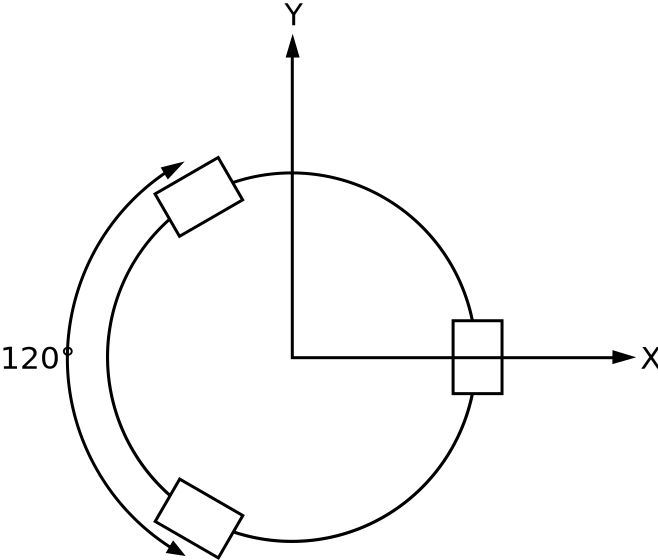
\includegraphics{figures/model}
	\caption{Modelo geometrico do robô de 3 rodas}
\end{figure}

\section{Matriz de translação}

\begin{gather}
	\begin{bmatrix} V_{w1} \\  V_{w2} \\  V_{w3} \end{bmatrix}
	=
	\begin{bmatrix}
		0 & 2/3 & L/3 \\
		-1/\sqrt{3} & -1/3 & L/3\\
		1/\sqrt{3} & -1/3 & L/3
	\end{bmatrix}
	\cdot
	\begin{bmatrix} V\cdot \cos{\theta} \\  V\cdot \sin{\theta} \\  \omega \end{bmatrix}
\end{gather}

\[ \overrightarrow{V} = (V\cos{\theta} , V\sin{\theta}) \]



\[\overrightarrow{V} \text{ :  Vetor velocidade linear do robô} \]  
\[V_{w1}   \text{ :  Velocidade linear da roda 1} \]  
\[V_{w2}   \text{ :  Velocidade linear da roda 2} \]  
\[V_{w3}   \text{ :  Velocidade linear da roda 3} \] 
\[\omega   \text{ :  Velocidade angular do robô a partir do centro de massa} \]  
\[L   \text{ :  Distância entre o centro de geometrico da roda e o centro de geometrico do robô} \]  



\section{Geometrica roda}

\[V_{w1} = \omega_{w1}\cdot r \]  
\[r   \text{ :  Raio da roda} \]  
\[\omega_{w1}   \text{ :  Velocidade angular da roda} \] 



	\chapter{Componentes}
	\input{chapters/capitulo_2.tex}

	\chapter{Outro Capítulo}
	
\section{Aliquam vestibulum fringilla lorem}


\lipsum[1]

\lipsum[2-3]


	% ----------------------------------------------------------
	% Finaliza a parte no bookmark do PDF
	% para que se inicie o bookmark na raiz
	% e adiciona espaço de parte no Sumário
	% ----------------------------------------------------------
	\phantompart


	% Conclusão
	\chapter{Conclusão}
% ---

\lipsum[1]


	

% ELEMENTOS PÓS-TEXTUAIS
\postextual

	% Referências bibliográficas
	\bibliography{abntex2-modelo-references}

	% Glossário
	\input{glossary/glossary_class.tex}

	% Apêndices
	\begin{apendicesenv}

% Imprime uma página indicando o início dos apêndices
\partapendices


\chapter{apendice 1}


\lipsum[1]

\chapter{apendice 2}

\lipsum[1]


\end{apendicesenv}

	% Anexos
	\begin{anexosenv}

% Imprime uma página indicando o início dos anexos
\partanexos


\begin{anexosenv}

\partanexos

\chapter{Cálculo modelo de 3 rodas}

\begin{figure}[h]
	\centering
	\includegraphics{figures/digram_model_dedution}
	\caption{diagrama do modelo - dedução da matriz}
	\label{lof}
\end{figure}

\begin{equation}
    \begin{split}
        \overrightarrow{V}_{l} = 
        \overrightarrow{V}_{w1}
        + \overrightarrow{V}_{w2}
        + \overrightarrow{V}_{w3}
    \end{split}
\end{equation}

\begin{equation}
    \begin{split}
        \overrightarrow{\omega} = 
        \frac{\vert\overrightarrow{V}_{w1}\vert}{L}
        + \frac{\vert\overrightarrow{V}_{w2}\vert}{L}
        + \frac{\vert\overrightarrow{V}_{w3}\vert}{L}
    \end{split}
\end{equation}


\begin{gather*}
        V_{l} \angle \theta =  
        V_{w1} \angle \left(-\frac{\pi}{2}\right) 
        + V_{w2} \angle \left(\frac{2\pi}{3}-\frac{\pi}{2}\right) 
        + V_{w3} \angle \left(\frac{4\pi}{3}-\frac{\pi}{2}\right) 
\end{gather*}

\begin{align*}
    V_{l} \cos{ \theta } + jV_{l} \sin{\theta} =  
    V_{w1} \cos{ \left(-\frac{\pi}{2}\right)} + jV_{w1} \sin{ \left(-\frac{\pi}{2}\right) } \\
    + V_{w2}  \cos{ \left(\frac{\pi}{6}\right) } + jV_{w2}  \sin{ \left(\frac{\pi}{6}\right) }  \\
    + V_{w3} \cos{ \left(\frac{5\pi}{6}\right) } + jV_{w2}  \sin{ \left(\frac{5\pi}{6}\right) } 
\end{align*}

\begin{equation*}
    \begin{split}
        \omega = 
        \frac{V_{w1}}{L}
        + \frac{V_{w2}}{L}
        + \frac{V_{w3}}{L}
    \end{split}
\end{equation*}


\begin{gather}
	\begin{bmatrix} V\cdot \cos{\theta} \\  V\cdot \sin{\theta} \\  \omega \end{bmatrix}
	=
	\begin{bmatrix}
		\cos{\left(-\frac{\pi}{2}\right)} & \cos{\left(\frac{\pi}{6}\right)} & \cos{\left(\frac{5\pi}{6}\right)} \\
		\sin{\left(-\frac{\pi}{2}\right)} & \sin{\left(\frac{\pi}{6}\right)} & \sin{\left(\frac{5\pi}{6}\right)} \\
		\frac{1}{L} & \frac{1}{L} & \frac{1}{L}
	\end{bmatrix}
	\cdot
	\begin{bmatrix} V_{w1} \\  V_{w2} \\  V_{w3} \end{bmatrix}
\end{gather}



\begin{gather}
	\begin{bmatrix} V_{w1} \\  V_{w2} \\  V_{w3} \end{bmatrix}
	=
	\begin{bmatrix}
		0 & 2/3 & L/3 \\
		-1/\sqrt{3} & -1/3 & L/3\\
		1/\sqrt{3} & -1/3 & L/3
	\end{bmatrix}
	\cdot
	\begin{bmatrix} V\cdot \cos{\theta} \\  V\cdot \sin{\theta} \\  \omega \end{bmatrix}
\end{gather}

\end{anexosenv}

\chapter{Outro Anexo}


\lipsum[32]



\end{anexosenv}



%---------------------------------------------------------------------
% INDICE REMISSIVO
%---------------------------------------------------------------------
\phantompart
\printindex


\end{document}